\chapter{Testprotokoll Sprint 2}
\section{Test}
\subsection{Angaben zum Test}

\begin{tabularx}{\linewidth}{l l l}
\textbf{datum des Builds} & \textbf{Tester} & \textbf{datum der Testdurchführung}\\
\hline
23.11.15 & Silvan Adrian & 23.11.15

\end{tabularx}

\subsection{Zusammenfassung Ergebnis}
\begin{tabularx}{\linewidth}{l l l}
\textbf{Test durchgeführt?} & \textbf{Tests erfolgreich?} & \textbf{Tests fehlgeschalgen?}\\
\hline
36 (alle) & 36 (alle) & 0 \\
\hline
\end{tabularx}


\subsection{Ergebnisse Tests}
\begin{tabularx}{\linewidth}{X l l}
\textbf{Was} & \textbf{Ok? / nicht OK?} & \textbf{Aufgetretene Fehler}\\
\hline
\textbf{Unit-Tests} & {\color{green} OK}  & keine\\
\hline
Systemtest 1: & & \\
\textbf{Service abonnieren} & {\color{green} OK} & keine\\
\hline
Systemtest 2: & & \\
\textbf{OrderedService kündigen} & {\color{green} OK}  & keine\\
\hline
Systemtest 3: & & \\
\textbf{Abonnierte Services anzeigen} & {\color{green} OK}  & keine\\
\hline
Systemtest 4: & & \\
\textbf{Verfügbare Services anzeigen} & {\color{green} OK}  & keine\\
\hline
Systemtest 5: & & \\
\textbf{ServiceModule, die einem Service zugeteilt sind anzeigen} & {\color{green} OK}  & keine\\
\hline
Systemtest 6: & & \\
\textbf{Abonnierter Service wird auf KVM Umgebung erstellt} & {\color{green} OK}  & keine\\
\hline
Systemtest 6: & & \\
\textbf{Gekündigter Service wird auf KVM Umgebung entfernt} & {\color{green} OK}  & keine\\
\hline



\end{tabularx}

\newpage

\section{Metriken}
Die abschliessenden Metriken vom Sprint aus SonarQube.
\subsection{Projekt in Zahlen}
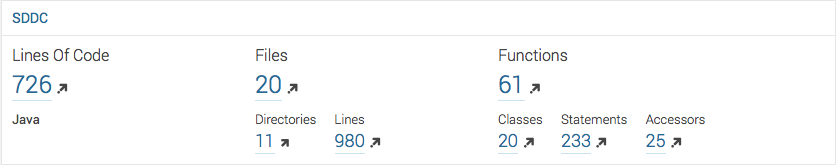
\includegraphics[width=\textwidth]{./10_Protokolle/04_Testprotokoll/images/Sprint2/loc}

\subsection{Unit Tests Coverage}
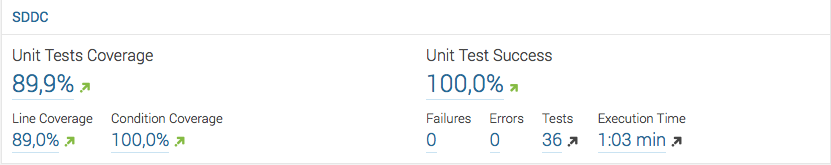
\includegraphics[width=\textwidth]{./10_Protokolle/04_Testprotokoll/images/Sprint2/coverage}

\subsection{Coverage Verteilung auf einzelne Dateien}
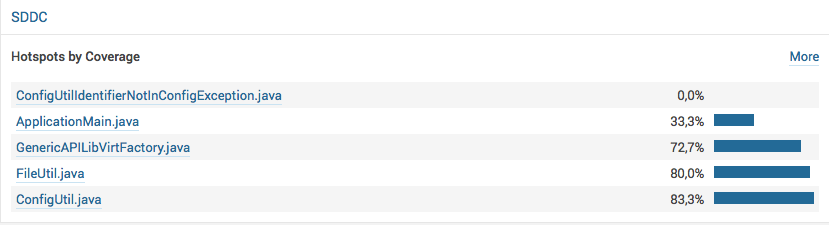
\includegraphics[width=\textwidth]{./10_Protokolle/04_Testprotokoll/images/Sprint2/coverageperfile}

\subsection{Findbugs Issues}
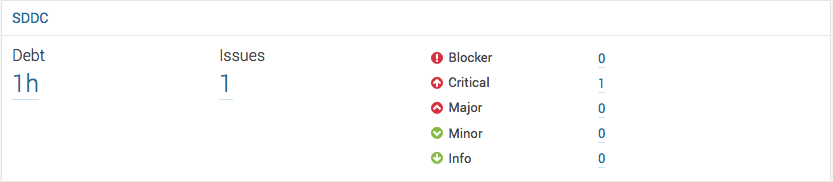
\includegraphics[width=\textwidth]{./10_Protokolle/04_Testprotokoll/images/Sprint2/issues}
\subsubsection{Issues}
\textbf{Incorrect Lazy Initialization}
\newline
Es handelt sich hierbei um ein Multithreading Problem, welches zulassen könnte 
das der Singleton mehrmals instanziert wird, da wir bisher noch keine bessere 
Möglichkeit gefunden haben um zwischen einzelnen ConnectionStrings zu 
unterscheiden wurde es so gelöst, im nächsten Sprint wird das Problem jedoch behoben.
\newline
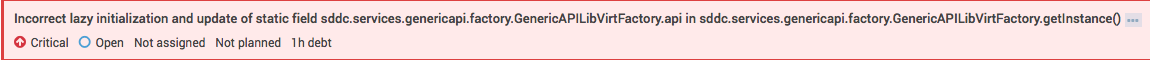
\includegraphics[width=\textwidth]{./10_Protokolle/04_Testprotokoll/images/Sprint2/lazy}

\section{Kommentare}

Die jetztige App bietet ein Customer Dashboard, auf welchem die Offerings und 
Services eingesehen werden können, dabei können bestehende Services (Ubuntu 14.04 und Debian7 etc.)
abonniert werden und werden auf unserer KVM Umgebung erstellt und bei Kündigung 
auch wieder gelöscht.
\newline
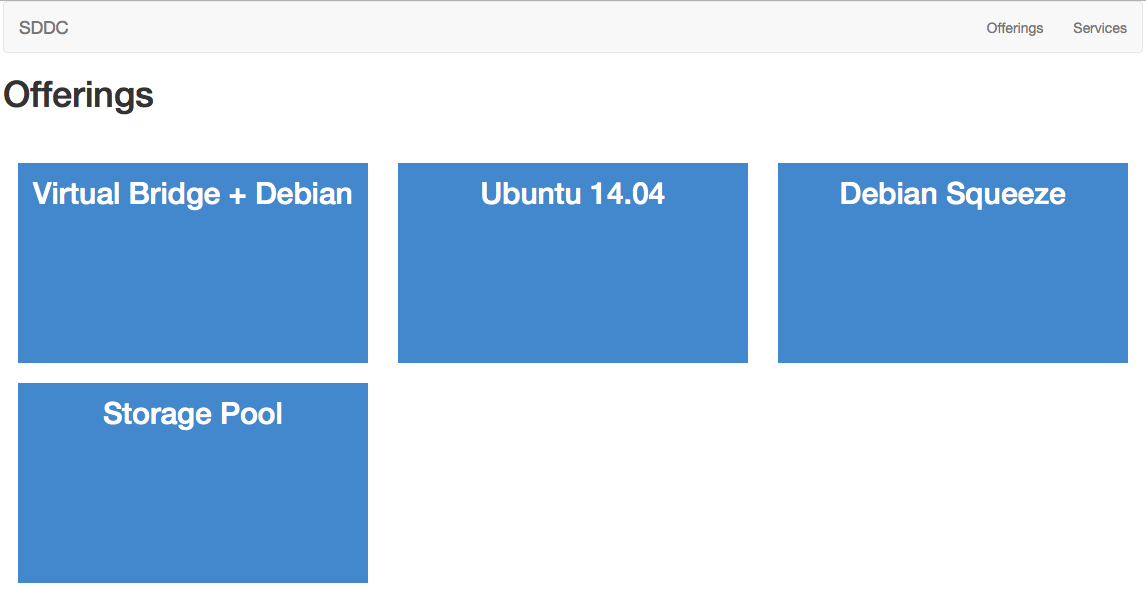
\includegraphics[width=\textwidth]{./10_Protokolle/04_Testprotokoll/images/Sprint2/dashboard}

